\documentclass{article}

\usepackage{arxiv}

\usepackage[utf8]{inputenc} % allow utf-8 input
\usepackage[T1]{fontenc}    % use 8-bit T1 fonts
\usepackage{lmodern}        % https://github.com/rstudio/rticles/issues/343
\usepackage{hyperref}       % hyperlinks
\usepackage{url}            % simple URL typesetting
\usepackage{booktabs}       % professional-quality tables
\usepackage{amsfonts}       % blackboard math symbols
\usepackage{nicefrac}       % compact symbols for 1/2, etc.
\usepackage{microtype}      % microtypography
\usepackage{graphicx}

\title{A Statistical Perspective of Non-Inferiority Trials}

\author{
  }

% Pandoc syntax highlighting
\usepackage{color}
\usepackage{fancyvrb}
\newcommand{\VerbBar}{|}
\newcommand{\VERB}{\Verb[commandchars=\\\{\}]}
\DefineVerbatimEnvironment{Highlighting}{Verbatim}{commandchars=\\\{\}}
% Add ',fontsize=\small' for more characters per line
\usepackage{framed}
\definecolor{shadecolor}{RGB}{248,248,248}
\newenvironment{Shaded}{\begin{snugshade}}{\end{snugshade}}
\newcommand{\AlertTok}[1]{\textcolor[rgb]{0.94,0.16,0.16}{#1}}
\newcommand{\AnnotationTok}[1]{\textcolor[rgb]{0.56,0.35,0.01}{\textbf{\textit{#1}}}}
\newcommand{\AttributeTok}[1]{\textcolor[rgb]{0.13,0.29,0.53}{#1}}
\newcommand{\BaseNTok}[1]{\textcolor[rgb]{0.00,0.00,0.81}{#1}}
\newcommand{\BuiltInTok}[1]{#1}
\newcommand{\CharTok}[1]{\textcolor[rgb]{0.31,0.60,0.02}{#1}}
\newcommand{\CommentTok}[1]{\textcolor[rgb]{0.56,0.35,0.01}{\textit{#1}}}
\newcommand{\CommentVarTok}[1]{\textcolor[rgb]{0.56,0.35,0.01}{\textbf{\textit{#1}}}}
\newcommand{\ConstantTok}[1]{\textcolor[rgb]{0.56,0.35,0.01}{#1}}
\newcommand{\ControlFlowTok}[1]{\textcolor[rgb]{0.13,0.29,0.53}{\textbf{#1}}}
\newcommand{\DataTypeTok}[1]{\textcolor[rgb]{0.13,0.29,0.53}{#1}}
\newcommand{\DecValTok}[1]{\textcolor[rgb]{0.00,0.00,0.81}{#1}}
\newcommand{\DocumentationTok}[1]{\textcolor[rgb]{0.56,0.35,0.01}{\textbf{\textit{#1}}}}
\newcommand{\ErrorTok}[1]{\textcolor[rgb]{0.64,0.00,0.00}{\textbf{#1}}}
\newcommand{\ExtensionTok}[1]{#1}
\newcommand{\FloatTok}[1]{\textcolor[rgb]{0.00,0.00,0.81}{#1}}
\newcommand{\FunctionTok}[1]{\textcolor[rgb]{0.13,0.29,0.53}{\textbf{#1}}}
\newcommand{\ImportTok}[1]{#1}
\newcommand{\InformationTok}[1]{\textcolor[rgb]{0.56,0.35,0.01}{\textbf{\textit{#1}}}}
\newcommand{\KeywordTok}[1]{\textcolor[rgb]{0.13,0.29,0.53}{\textbf{#1}}}
\newcommand{\NormalTok}[1]{#1}
\newcommand{\OperatorTok}[1]{\textcolor[rgb]{0.81,0.36,0.00}{\textbf{#1}}}
\newcommand{\OtherTok}[1]{\textcolor[rgb]{0.56,0.35,0.01}{#1}}
\newcommand{\PreprocessorTok}[1]{\textcolor[rgb]{0.56,0.35,0.01}{\textit{#1}}}
\newcommand{\RegionMarkerTok}[1]{#1}
\newcommand{\SpecialCharTok}[1]{\textcolor[rgb]{0.81,0.36,0.00}{\textbf{#1}}}
\newcommand{\SpecialStringTok}[1]{\textcolor[rgb]{0.31,0.60,0.02}{#1}}
\newcommand{\StringTok}[1]{\textcolor[rgb]{0.31,0.60,0.02}{#1}}
\newcommand{\VariableTok}[1]{\textcolor[rgb]{0.00,0.00,0.00}{#1}}
\newcommand{\VerbatimStringTok}[1]{\textcolor[rgb]{0.31,0.60,0.02}{#1}}
\newcommand{\WarningTok}[1]{\textcolor[rgb]{0.56,0.35,0.01}{\textbf{\textit{#1}}}}

% tightlist command for lists without linebreak
\providecommand{\tightlist}{%
  \setlength{\itemsep}{0pt}\setlength{\parskip}{0pt}}

% From pandoc table feature
\usepackage{longtable,booktabs,array}
\usepackage{calc} % for calculating minipage widths
% Correct order of tables after \paragraph or \subparagraph
\usepackage{etoolbox}
\makeatletter
\patchcmd\longtable{\par}{\if@noskipsec\mbox{}\fi\par}{}{}
\makeatother
% Allow footnotes in longtable head/foot
\IfFileExists{footnotehyper.sty}{\usepackage{footnotehyper}}{\usepackage{footnote}}
\makesavenoteenv{longtable}

% Pandoc citation processing
%From Pandoc 3.1.8
% definitions for citeproc citations
\NewDocumentCommand\citeproctext{}{}
\NewDocumentCommand\citeproc{mm}{%
  \begingroup\def\citeproctext{#2}\cite{#1}\endgroup}
\makeatletter
 % allow citations to break across lines
 \let\@cite@ofmt\@firstofone
 % avoid brackets around text for \cite:
 \def\@biblabel#1{}
 \def\@cite#1#2{{#1\if@tempswa , #2\fi}}
\makeatother
\newlength{\cslhangindent}
\setlength{\cslhangindent}{1.5em}
\newlength{\csllabelwidth}
\setlength{\csllabelwidth}{3em}
\newenvironment{CSLReferences}[2] % #1 hanging-indent, #2 entry-spacing
 {\begin{list}{}{%
  \setlength{\itemindent}{0pt}
  \setlength{\leftmargin}{0pt}
  \setlength{\parsep}{0pt}
  % turn on hanging indent if param 1 is 1
  \ifodd #1
   \setlength{\leftmargin}{\cslhangindent}
   \setlength{\itemindent}{-1\cslhangindent}
  \fi
  % set entry spacing
  \setlength{\itemsep}{#2\baselineskip}}}
 {\end{list}}
\usepackage{calc}
\newcommand{\CSLBlock}[1]{#1\hfill\break}
\newcommand{\CSLLeftMargin}[1]{\parbox[t]{\csllabelwidth}{#1}}
\newcommand{\CSLRightInline}[1]{\parbox[t]{\linewidth - \csllabelwidth}{#1}\break}
\newcommand{\CSLIndent}[1]{\hspace{\cslhangindent}#1}

\begin{document}
\maketitle


\begin{abstract}
Single-arm performance goal studies are widely used in medical device
evaluation when a randomised active-control trial is impractical or
ethically unjustifiable. In this setting, the trial conclusion depends
on whether a confidence interval for the observed event proportion
satisfies a pre-specified benchmark derived from historical evidence.
Despite their apparent simplicity, the conclusions of such studies are
sensitive to three interconnected methodological choices: the value of
the performance goal, the confidence interval method used to construct
the decision rule, and the sample size calculation underlying the study
design. This thesis examines each of these choices in the context of a
retrospective case study of the BioMimics 3D vascular stent, a helical
nitinol stent developed for the treatment of femoropopliteal peripheral
artery disease.Performance goals for a 30-day composite safety endpoint
and a 12-month Rutherford classification efficacy endpoint were derived
through a generalised linear mixed model meta-analysis of three
historical femoropopliteal bare nitinol stent studies comprising 116
patients in total. Using confidence interval boundaries rather than
point estimates to account for uncertainty in the historical evidence
yielded a maximum acceptable 30-day composite adverse event rate of 12\%
and a minimum acceptable 12-month Rutherford success proportion of 88\%.
The limited evidence base produced wide uncertainty around both
estimates, illustrating that performance goals carry inherent
uncertainty that is not always visible when they are reported as fixed
values. A simulation study evaluated six confidence interval methods for
binary proportions across a grid of true event proportions and sample
sizes relevant to the case study endpoints. The Wald interval was the
only method to consistently fall below the nominal 95\% coverage level
and was judged unsuitable as a decision tool in this setting. Among the
remaining methods, Wilson Score and Jeffreys achieved coverage closest
to the nominal level with the narrowest intervals, while
Clopper-Pearson, Agresti-Coull and the continuity-corrected Wilson Score
were conservative with progressively wider intervals. These differences
in coverage behaviour translated into meaningful differences in sample
size requirements. Under an approved performance goal of 11\%, an
assumed true complication proportion of 5\% and a target power of 90\%,
Clopper-Pearson was used as the primary method, requiring 209 evaluable
patients at 89.7\% achieved power. Among methods meeting the nominal
coverage level, the required sample size ranged from 198 patients under
Jeffreys to 247 under the continuity-corrected Wilson Score. A Bayesian
historical borrowing analysis demonstrated that incorporating prior
evidence through a Beta(2, 48) prior reduced the required sample size
from 209 to 79 patients, a reduction of approximately 62\%. This
reduction was sensitive to the weight assigned to the prior, with
stronger borrowing increasing dependence on the exchangeability
assumption and the risk of inflating the Type I error rate when
historical and current populations are not sufficiently comparable. An
interactive R Shiny application, PG-Power, was developed to implement
the sample size framework and make the sensitivity of required sample
size to key design assumptions accessible and reproducible. The
application supports confidence interval method comparison, power curve
visualisation, sensitivity analysis and report generation for single-arm
performance goal studies. The findings demonstrate that the performance
goal value, confidence interval method and sample size procedure are not
independent design choices and that each can alter the conclusion of a
performance goal study independently of the underlying clinical data.
Transparent derivation and pre-specification of these choices in the SAP
is essential to the credibility and reproducibility of performance goal
studies in medical device evaluation.
\end{abstract}

\keywords{
    binomial confidence intervals
   \and
    performance goals
   \and
    single-arm clinical trials
   \and
    medical device evaluation
   \and
    sample size calculation
   \and
    Bayesian historical borrowing
  }

\section{1. Introduction}\label{introduction}

\subsection{1.1 Non-inferiority Trials}\label{non-inferiority-trials}

Non-inferiority trials arise when an effective treatment or device
already exists and a placebo-controlled comparison would be unethical,
impractical or clinically uninformative(1--3). Rather than demonstrating
superiority, the goal is to show that any loss of efficacy associated
with the new intervention remains within a clinically acceptable
limit(1--3). This limit, known as the non-inferiority margin, represents
the largest reduction in efficacy considered tolerable in exchange for
other benefits such as improved safety, simpler delivery, lower cost or
better patient adherence(1,2,4). The trial conclusion depends on both
the observed treatment effect and the uncertainty surrounding it(1,2,5).
In practice, this is assessed by comparing a confidence interval for the
treatment effect against the pre-specified margin(1,2,6). For favourable
endpoints, where higher values indicate better performance, the lower
confidence bound is the relevant quantity, while for unfavourable
endpoints the upper bound is used(1,2). This one-sided structure
distinguishes non-inferiority trials from superiority and equivalence
designs, and places the choice of margin and confidence interval method
at the centre of the trial's interpretation(1--3,6).

\subsection{1.2 Performance Goals in Medical Device
Studies}\label{performance-goals-in-medical-device-studies}

Performance goal studies are closely related to non-inferiority designs
and are particularly common in medical device evaluation(1,7,8). Rather
than comparing the new intervention against an active control, the
observed outcome is compared with a pre-specified benchmark derived from
historical evidence and clinical judgement(7,9). This benchmark defines
the minimum level of performance considered acceptable for the device
under evaluation(7,9). The performance goal approach is most useful when
a randomised active-control trial is difficult to justify or
conduct(7,8). However, the absence of a concurrent comparator makes the
choice of benchmark especially consequential(7,10). Historical studies
may differ from the current trial in ways that affect the validity of
the comparison, including differences in the target population, endpoint
definitions, follow-up duration and broader clinical practice(7,10).
These differences must be carefully considered when constructing and
justifying a performance goal. The direction of the performance goal
depends on the nature of the endpoint(7,9). For efficacy endpoints,
where higher event proportions reflect better performance, the estimated
proportion and its confidence interval must exceed a minimum acceptable
level(7,9). For safety endpoints, where lower proportions are desirable,
the estimated proportion and its confidence interval must remain below a
maximum acceptable level of harm(7,9). In either case, a performance
goal should not be treated as a simple numerical cut-off(5,7,9). It
represents a clinical and statistical threshold whose validity depends
on the endpoint being measured, the quality and consistency of the
historical evidence, and the level of uncertainty considered acceptable
for regulatory decision-making(7,8,10).

\subsection{1.3 Motivation for Study}\label{motivation-for-study}

Although non-inferiority and performance goal designs appear
straightforward in principle, their conclusions can be sensitive to
several methodological choices(1--3). Small variations in any of these
decisions can alter the interpretation of the same clinical data and,
consequently, the study conclusion(1,2). This sensitivity is
particularly consequential in medical device studies, where single-arm
performance goal designs are common and the absence of a concurrent
comparator means the historical benchmark carries much of the evidential
weight(7,8,11). If the benchmark is too lenient, a device may appear
acceptable despite a clinically meaningful loss of performance. If it is
too strict, a device that performs well may require an impractically
large sample size or fail to meet the criterion regardless(4,7,10). In
either case, the benchmark itself shapes the conclusion before a single
patient is enrolled. Previous reviews have raised concerns about how
consistently these choices are reported. Piaggio et al.~found that only
around one-fifth of 332 non-inferiority and equivalence trials published
between 1990 and 2000 provided a suitable rationale for the chosen
margin(6). A later review of 232 drug trials found that while nearly all
reports specified a margin, only 24\% explained how it had been
determined(6). Together these findings point to a recurring problem:
margins and performance goals are often presented as settled values
without making the reasoning behind them transparent(2,6). This study is
motivated by that problem. Using the BioMimics 3D vascular stent trial
as a case study, it examines how performance goal selection, confidence
interval choice and sample size calculation interact to influence
conclusions in a single-arm medical device setting(1,5--7).

\subsection{1.4 Case Study: Biomimics 3D Vascular
Stent}\label{case-study-biomimics-3d-vascular-stent}

The BioMimics 3D vascular stent trial serves as the primary case study
throughout this analysis. Rather than attempting to reproduce the
original trial, the case study is used as a real medical device setting
in which to examine how statistical choices surrounding performance
goals influence the interpretation of device performance. Clinical and
regulatory context for the analysis was obtained through meetings with a
lead scientist involved in the original trial. These discussions
clarified how the device was intended to be evaluated in practice and
highlighted that the statistical design could not be reduced to a purely
numerical exercise- it had to reflect clinical judgement, regulatory
expectations and practical feasibility alongside the available evidence.

\subsection{1.5 Study Aims}\label{study-aims}

This study has five objectives:

\begin{enumerate}
\def\labelenumi{\arabic{enumi}.}
\tightlist
\item
  To derive evidence-based performance goals for a single-arm medical
  device study through meta-analysis of comparable historical device
  studies;
\item
  To compare confidence interval methods for binary endpoints in terms
  of coverage probability and interval width;
\item
  To evaluate how performance goal selection and confidence interval
  choice affect sample size requirements and non-inferiority
  conclusions;
\item
  To develop an interactive Shiny application, PG-Power, to support
  sample size planning and confidence interval method selection in
  performance goal studies;
\item
  To explore the potential role of Bayesian historical borrowing as a
  means of reducing the required sample size.
\end{enumerate}

\section{2. Background and Statistical
Framework}\label{background-and-statistical-framework}

\subsection{2.1 Superiority, Equivalence and
Non-Inferiority}\label{superiority-equivalence-and-non-inferiority}

Superiority, equivalence and non-inferiority trials address distinct
clinical questions and should not be interpreted interchangeably(12,13).
Let p\_Tdenote the success probability in the investigational treatment
group and p\_Cdenote the success probability in the comparator group.
For a binary success endpoint, the treatment effect is defined
as(13,14):

\[\theta = p_T - p_C\]

A superiority trial evaluates whether the investigational treatment
performs better than the comparator. The null and alternative hypotheses
are(1,12,13):

\[H_0: \theta \leq 0 \qquad H_1: \theta > 0\] Superiority is concluded
when the lower confidence bound for θ lies above zero(1).

An equivalence trial asks whether the difference between treatments is
small enough to be considered clinically unimportant in either
direction. Denoting the equivalence margin as \[Δ_E\], the hypotheses
are(6,12,13)

\[H_0: \theta \leq -\Delta_E \text{ or } \theta \geq \Delta_E \qquad H_1: -\Delta_E < \theta < \Delta_E\]

Equivalence is concluded when the confidence interval for θ lies
entirely within the equivalence margins(6,12,13):

\[-\Delta_E < \text{CI}_{1-\alpha}(\theta) < \Delta_E\]

A non-inferiority trial is less restrictive, focusing only on
differences in the unfavourable direction. Denoting the non-inferiority
margin as Δ\_NI, the largest clinically acceptable loss of efficacy, the
hypotheses are(1,2,12,13):

\[H_0: \theta \leq -\Delta_{NI} \qquad H_1: \theta > -\Delta_{NI}\]

Non-inferiority is concluded when the lower confidence bound lies above
the margin(1,6,12,13):

\[L_{1-\alpha}(\theta) > -\Delta_{NI}\]

These three designs are often confused in practice, but the distinction
matters. Failure to demonstrate superiority does not imply equivalence
or non-inferiority- a non-significant superiority test may simply
reflect insufficient power or imprecision rather than genuine similarity
between treatments(1,2,12). Each design therefore requires its own
pre-specified margin, endpoints, analysis population and decision rule,
and conclusions should not be switched between frameworks after the data
have been collected(5,6,13).

\section{Headings: first level}\label{headings-first-level}

\label{sec:headings}

You can use directly LaTeX command or Markdown text.

LaTeX command can be used to reference other section. See Section
\ref{sec:headings}. However, you can also use \textbf{bookdown}
extensions mechanism for this.

\subsection{Headings: second level}\label{headings-second-level}

You can use equation in blocks

\[
\xi _{ij}(t)=P(x_{t}=i,x_{t+1}=j|y,v,w;\theta)= {\frac {\alpha _{i}(t)a^{w_t}_{ij}\beta _{j}(t+1)b^{v_{t+1}}_{j}(y_{t+1})}{\sum _{i=1}^{N} \sum _{j=1}^{N} \alpha _{i}(t)a^{w_t}_{ij}\beta _{j}(t+1)b^{v_{t+1}}_{j}(y_{t+1})}}
\]

But also inline i.e \(z=x+y\)

\subsubsection{Headings: third level}\label{headings-third-level}

Another paragraph.

\section{Examples of citations, figures, tables,
references}\label{examples-of-citations-figures-tables-references}

\label{sec:others}

You can insert references. Here is some text (Kour and Saabne 2014b,
2014a) and see Hadash et al. (2018).

The documentation for \verb+natbib+ may be found at

You can use custom blocks with LaTeX support from \textbf{rmarkdown} to
create environment.

\begin{center}
\url{http://mirrors.ctan.org/macros/latex/contrib/natbib/natnotes.pdf\%7D}

\end{center}

Of note is the command \verb+\citet+, which produces citations
appropriate for use in inline text.

You can insert LaTeX environment directly too.

\begin{verbatim}
   \citet{hasselmo} investigated\dots
\end{verbatim}

produces

\begin{quote}
  Hasselmo, et al.\ (1995) investigated\dots
\end{quote}

\begin{center}
  \url{https://www.ctan.org/pkg/booktabs}
\end{center}

\subsection{Figures}\label{figures}

You can insert figure using LaTeX directly.

See Figure \ref{fig:fig1}. Here is how you add footnotes. {[}\^{}Sample
of the first footnote.{]}

\begin{figure}
  \centering
  \fbox{\rule[-.5cm]{4cm}{4cm} \rule[-.5cm]{4cm}{0cm}}
  \caption{Sample figure caption.}
  \label{fig:fig1}
\end{figure}

But you can also do that using R.

\begin{Shaded}
\begin{Highlighting}[]
\FunctionTok{plot}\NormalTok{(mtcars}\SpecialCharTok{$}\NormalTok{mpg)}
\end{Highlighting}
\end{Shaded}

\begin{figure}
\centering
\pandocbounded{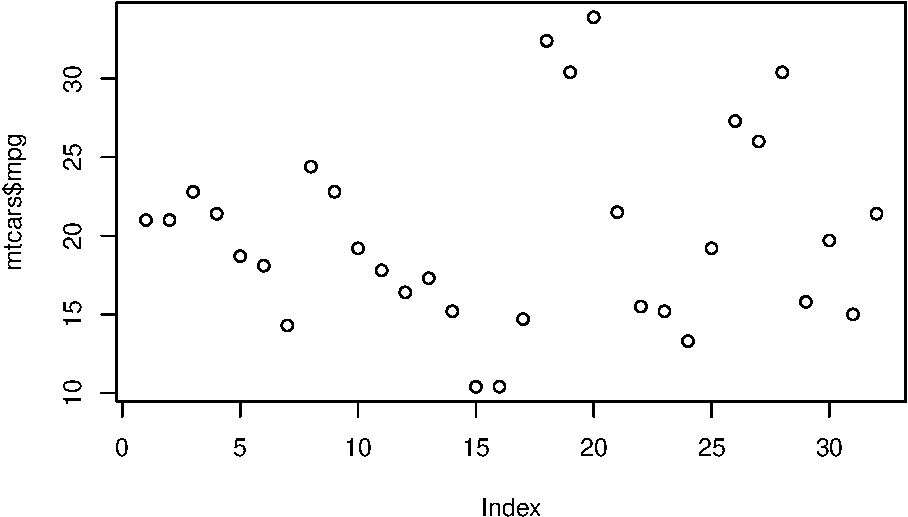
\includegraphics[keepaspectratio]{Untitled_files/figure-latex/fig2-1.pdf}}
\caption{Another sample figure}
\end{figure}

You can use \textbf{bookdown} to allow references for Tables and
Figures.

\subsection{Tables}\label{tables}

Below we can see how to use tables.

See awesome Table\textasciitilde{}\ref{tab:table} which is written
directly in LaTeX in source Rmd file.

\begin{table}
 \caption{Sample table title}
  \centering
  \begin{tabular}{lll}
    \toprule
    \multicolumn{2}{c}{Part}                   \\
    \cmidrule(r){1-2}
    Name     & Description     & Size ($\mu$m) \\
    \midrule
    Dendrite & Input terminal  & $\sim$100     \\
    Axon     & Output terminal & $\sim$10      \\
    Soma     & Cell body       & up to $10^6$  \\
    \bottomrule
  \end{tabular}
  \label{tab:table}
\end{table}

You can also use R code for that.

\begin{Shaded}
\begin{Highlighting}[]
\NormalTok{knitr}\SpecialCharTok{::}\FunctionTok{kable}\NormalTok{(}\FunctionTok{head}\NormalTok{(mtcars), }\AttributeTok{caption =} \StringTok{"Head of mtcars table"}\NormalTok{)}
\end{Highlighting}
\end{Shaded}

\begin{longtable}[]{@{}
  >{\raggedright\arraybackslash}p{(\linewidth - 22\tabcolsep) * \real{0.2609}}
  >{\raggedleft\arraybackslash}p{(\linewidth - 22\tabcolsep) * \real{0.0725}}
  >{\raggedleft\arraybackslash}p{(\linewidth - 22\tabcolsep) * \real{0.0580}}
  >{\raggedleft\arraybackslash}p{(\linewidth - 22\tabcolsep) * \real{0.0725}}
  >{\raggedleft\arraybackslash}p{(\linewidth - 22\tabcolsep) * \real{0.0580}}
  >{\raggedleft\arraybackslash}p{(\linewidth - 22\tabcolsep) * \real{0.0725}}
  >{\raggedleft\arraybackslash}p{(\linewidth - 22\tabcolsep) * \real{0.0870}}
  >{\raggedleft\arraybackslash}p{(\linewidth - 22\tabcolsep) * \real{0.0870}}
  >{\raggedleft\arraybackslash}p{(\linewidth - 22\tabcolsep) * \real{0.0435}}
  >{\raggedleft\arraybackslash}p{(\linewidth - 22\tabcolsep) * \real{0.0435}}
  >{\raggedleft\arraybackslash}p{(\linewidth - 22\tabcolsep) * \real{0.0725}}
  >{\raggedleft\arraybackslash}p{(\linewidth - 22\tabcolsep) * \real{0.0725}}@{}}
\caption{Head of mtcars table}\tabularnewline
\toprule\noalign{}
\begin{minipage}[b]{\linewidth}\raggedright
\end{minipage} & \begin{minipage}[b]{\linewidth}\raggedleft
mpg
\end{minipage} & \begin{minipage}[b]{\linewidth}\raggedleft
cyl
\end{minipage} & \begin{minipage}[b]{\linewidth}\raggedleft
disp
\end{minipage} & \begin{minipage}[b]{\linewidth}\raggedleft
hp
\end{minipage} & \begin{minipage}[b]{\linewidth}\raggedleft
drat
\end{minipage} & \begin{minipage}[b]{\linewidth}\raggedleft
wt
\end{minipage} & \begin{minipage}[b]{\linewidth}\raggedleft
qsec
\end{minipage} & \begin{minipage}[b]{\linewidth}\raggedleft
vs
\end{minipage} & \begin{minipage}[b]{\linewidth}\raggedleft
am
\end{minipage} & \begin{minipage}[b]{\linewidth}\raggedleft
gear
\end{minipage} & \begin{minipage}[b]{\linewidth}\raggedleft
carb
\end{minipage} \\
\midrule\noalign{}
\endfirsthead
\toprule\noalign{}
\begin{minipage}[b]{\linewidth}\raggedright
\end{minipage} & \begin{minipage}[b]{\linewidth}\raggedleft
mpg
\end{minipage} & \begin{minipage}[b]{\linewidth}\raggedleft
cyl
\end{minipage} & \begin{minipage}[b]{\linewidth}\raggedleft
disp
\end{minipage} & \begin{minipage}[b]{\linewidth}\raggedleft
hp
\end{minipage} & \begin{minipage}[b]{\linewidth}\raggedleft
drat
\end{minipage} & \begin{minipage}[b]{\linewidth}\raggedleft
wt
\end{minipage} & \begin{minipage}[b]{\linewidth}\raggedleft
qsec
\end{minipage} & \begin{minipage}[b]{\linewidth}\raggedleft
vs
\end{minipage} & \begin{minipage}[b]{\linewidth}\raggedleft
am
\end{minipage} & \begin{minipage}[b]{\linewidth}\raggedleft
gear
\end{minipage} & \begin{minipage}[b]{\linewidth}\raggedleft
carb
\end{minipage} \\
\midrule\noalign{}
\endhead
\bottomrule\noalign{}
\endlastfoot
Mazda RX4 & 21.0 & 6 & 160 & 110 & 3.90 & 2.620 & 16.46 & 0 & 1 & 4 &
4 \\
Mazda RX4 Wag & 21.0 & 6 & 160 & 110 & 3.90 & 2.875 & 17.02 & 0 & 1 & 4
& 4 \\
Datsun 710 & 22.8 & 4 & 108 & 93 & 3.85 & 2.320 & 18.61 & 1 & 1 & 4 &
1 \\
Hornet 4 Drive & 21.4 & 6 & 258 & 110 & 3.08 & 3.215 & 19.44 & 1 & 0 & 3
& 1 \\
Hornet Sportabout & 18.7 & 8 & 360 & 175 & 3.15 & 3.440 & 17.02 & 0 & 0
& 3 & 2 \\
Valiant & 18.1 & 6 & 225 & 105 & 2.76 & 3.460 & 20.22 & 1 & 0 & 3 & 1 \\
\end{longtable}

\subsection{Lists}\label{lists}

\begin{itemize}
\tightlist
\item
  Item 1
\item
  Item 2
\item
  Item 3
\end{itemize}

\phantomsection\label{refs}
\begin{CSLReferences}{1}{0}
\bibitem[\citeproctext]{ref-hadash2018estimate}
Hadash, Guy, Einat Kermany, Boaz Carmeli, Ofer Lavi, George Kour, and
Alon Jacovi. 2018. {``Estimate and Replace: A Novel Approach to
Integrating Deep Neural Networks with Existing Applications.''}
\emph{arXiv Preprint arXiv:1804.09028}.

\bibitem[\citeproctext]{ref-kour2014fast}
Kour, George, and Raid Saabne. 2014a. {``Fast Classification of
Handwritten on-Line Arabic Characters.''} In \emph{Soft Computing and
Pattern Recognition (SoCPaR), 2014 6th International Conference of},
312--18. IEEE.

\bibitem[\citeproctext]{ref-kour2014real}
---------. 2014b. {``Real-Time Segmentation of on-Line Handwritten
Arabic Script.''} In \emph{Frontiers in Handwriting Recognition (ICFHR),
2014 14th International Conference on}, 417--22. IEEE.

\end{CSLReferences}

\bibliographystyle{unsrt}
\bibliography{references.bib}


\end{document}
